\chapter{Learning Rules With Numerical and Categorical Attributes}
\label{cl:intro}

In this chapter, we describe the kind of rules we are interested in, define categorical properties,
describe in more details a correlation lattice, how to build it and integrate it into the core ILP learning
algorithm.

\section{Interesting Rule Definition}

In this section, we formally define the kind of rules we are interested in. As briefly explained in the introduction,
the objective is to learn rules with numerical properties, focusing on searching intervals in the numerical attribute's
domain that satisfy support and confidence thresholds.

In this context, we define a rule with a free numerical variable as a \emph{base-rule} and the same rule with the
numerical variable restricted to a specific interval as a \emph{refined-rule}. For instance, if we have
two rules $r_1$ and $r_2$:

\begin{align*}
r_1: employmentStatus(X,unemployed)&\text{ :- }hasIncome(X,Y) \\
r_2: employmentStatus(X,unemployed)&\text{ :- }hasIncome(X,Y),Y>100000
\end{align*}

then we say that $r_1$ is the base-rule of $r_2$, and $r_2$ is a refined-rule of $r_1$.

Searching numerical intervals for a base-rule that already satisfies the confidence threshold is usually not
interesting, since the base-rule itself already covers the whole numerical attribute
domain. Moreover, even if for some specific interval we have a higher confidence value, the gain in comparison to
its base-rule would not be very significant, since the base-rule already presents a fairly high confidence value.

More precisely, if we have a confidence threshold $minConf$, and define confidence gain from a refined-rule
$r_2$ in comparison to its base-rule $r_1$, $gain_{r_2,r_1}$ as:

\begin{equation}
 gain_{r_2,r1}=\cfrac{conf_{r_2}}{conf_{r_1}}
\label{eq:gain}
\end{equation}

since $r_1 \geq minConf$, then $gain_{r_2,r_1}$ is upper-bounded by:

\begin{equation}
 gain_{r_2,r1} \leq \cfrac{1}{minConf}
\end{equation}

Therefore, we interesting in base-rules which satisfy the support threshold but do not satisfy the
confidence threshold. In this case, if we the confidence distribution along the buckets is non-uniform, it is possible
to find a refined-rule that satisfies both thresholds, and potentially has a significant confidence gain.

In Figure~\ref{interestingnessExample}, we illustrate that a rule whose positive examples and body
support have completely different distributions, and therefore, has a very interesting confidence distribution. This
happens because of the divergent distributions of positives (examples that satisfy the head
and body) and body support (examples that support the body). This is emphasized in
Figure~\ref{interestingnessDistribution}, where we show the distributions obtained by normalizing the frequency
histograms of Figure~\ref{interestingnessExample} (left).

\begin{figure} [h!]
  \caption{Example of frequency histograms from body support and positives support (left), and resulting confidence
distribution (right)}
  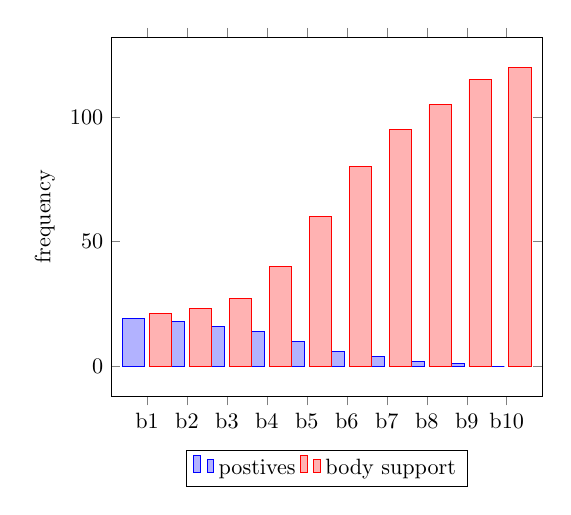
\begin{tikzpicture}[scale=0.8]
  \begin{axis}[
      ybar,
      enlargelimits=0.10,
      legend style={at={(0.5,-0.15)},
	anchor=north,legend columns=-1},
      ylabel={frequency},
      symbolic x coords={b1,b2,b3,b4,b5,b6,b7,b8,b9,b10},
      xtick=data,
      %nodes near coords,
      %nodes near coords align={vertical},
      %every node near coord/.append style={ anchor=mid west, rotate=70 },
      ]
  \addplot coordinates 
     {(b1,19) (b2,18) (b3,16) (b4,14) (b5,10) (b6,6) (b7,4) (b8,2) (b9,1) (b10,0)};
  \addplot coordinates
     {(b1,21) (b2,23) (b3,27) (b4,40) (b5,60) (b6,80) (b7,95) (b8,105) (b9,115) (b10,120)};
  \legend{postives, body support}
  \end{axis}
  \end{tikzpicture}
  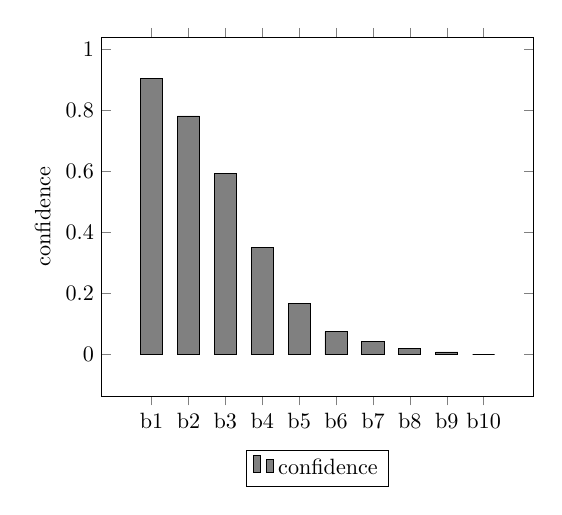
\begin{tikzpicture}[scale=0.8]
  \begin{axis}[
      ybar,
      enlargelimits=0.15,
      legend style={at={(0.5,-0.15)},
	anchor=north,legend columns=-1},
      ylabel={confidence},
      yticklabel={},
      symbolic x coords={b1,b2,b3,b4,b5,b6,b7,b8,b9,b10},
      xtick=data,
      %nodes near coords,
      %nodes near coords align={vertical},
      %every node near coord/.append style={ anchor=mid west, rotate=70 },
      ]
  \addplot[fill=gray] coordinates
     {(b1,0.904761904761905)
      (b2,0.782608695652174)
      (b3,0.592592592592593)
      (b4,0.35)
      (b5,0.166666666666667)
      (b6,0.075)
      (b7,0.0421052631578947)
      (b8,0.019047619047619)
      (b9,0.00869565217391304)
      (b10,0)};
  \legend{confidence}
  \end{axis}
  \end{tikzpicture}
  \label{interestingnessExample} 
\end{figure}


\begin{figure}[h!]
\begin{center}
  \caption{Support distribution of body and positives from figure~\ref{interestingnessExample}}
  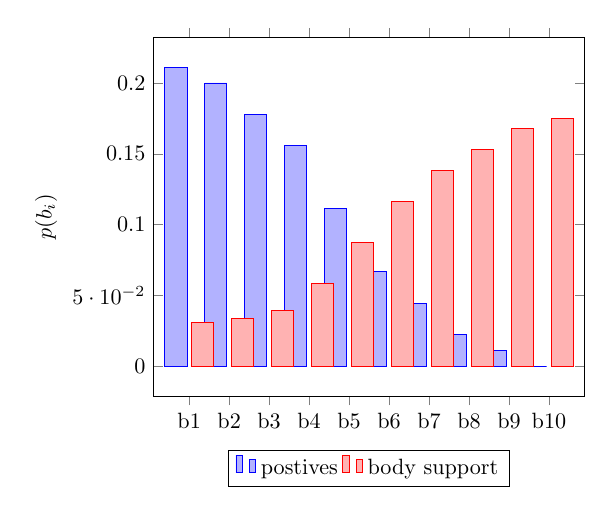
\begin{tikzpicture}[scale=0.8]
  \begin{axis}[
      ybar,
      enlargelimits=0.10,
      legend style={at={(0.5,-0.15)},
	anchor=north,legend columns=-1},
      ylabel={$p(b_i)$},
      symbolic x coords={b1,b2,b3,b4,b5,b6,b7,b8,b9,b10},
      xtick=data,
      %nodes near coords,
      %nodes near coords align={vertical},
      ]
  \addplot coordinates
     {(b1,0.211111111111111)
      (b2,0.2)
      (b3,0.177777777777778)
      (b4,0.155555555555556)
      (b5,0.111111111111111)
      (b6,0.0666666666666667)
      (b7,0.0444444444444444)
      (b8,0.0222222222222222)
      (b9,0.0111111111111111)
      (b10,0)};
  \addplot coordinates
     {(b1,0.0306122448979592)
      (b2,0.0335276967930029)
      (b3,0.0393586005830904)
      (b4,0.0583090379008746)
      (b5,0.0874635568513119)
      (b6,0.116618075801749)
      (b7,0.138483965014577)
      (b8,0.153061224489796)
      (b9,0.167638483965015)
      (b10,0.174927113702624)};
  \legend{postives, body support}
  \end{axis}
  \end{tikzpicture}
\label{interestingnessDistribution}
\end{center}
\end{figure}

\section{Categorical Property Definition}
\label{sec:categorical-properties}

In this section we formally define the categorical properties used in the correlation lattice. First of all, it is
important to mention that a correlation lattice has a root's numerical property. This numerical property is supposed to
have a numerical attribute $Y$, and a non-numerical attribute $X \in \mathcal{X}$, which serves as join variable.

A property $r(X,Z)$ is categorical if the variable $Z$ is within a categorical domain $\mathcal{Z}$ with a finite
number of categories $\{z_1,z_2,\ldots,z_n\}$. Moreover, for being included in the correlation lattice, this
property should be joinable with the root's join variable. As a result, this property should be able to generate
categorical sub-populations of $\mathcal{X}$:

\begin{center}
$\mathcal{X}_{z_i}= \{ x | x \in \mathcal{X} \wedge \exists r(x,z_i) \}$ 
\end{center}

where typically, $|\mathcal{X}| \gg n$ and  $|\mathcal{X}_{z_i}| < |\mathcal{X}|$.

\begin{table}[h!]
 \begin{center}
 \caption{Example data for categorical relation $hasSex$}
  \begin{tabular}{*{2}{l}}
    \toprule
    hasIncome(john,20000) & hasSex(john,male) 	\\
    hasIncome(mike,30000) & hasSex(mike,male) 	\\
    hasIncome(anne,25000) & hasSex(anne,female) 	\\
    hasIncome(mary,5000)  & hasSex(mary,female) 	\\
    hasIncome(lisa,10000) & hasSex(lisa,female)	\\
    hasIncome(paul,0)	  & hasSex(paul,male)	\\
    \bottomrule
  \end{tabular}
 \label{tab:cat1}
 \end{center}

\end{table}
  
For the example shown in Table~\ref{tab:cat1}, if we define $\mathcal{X}=\{ x|\exists hasIncome(x,Y), Y \in \mathcal{Y}
\}$, then we can split $\mathcal{X}$ into the following categories:

\begin{align*}
 \mathcal{X}_{male}&=\{ x|x \in \mathcal{X} \wedge \exists hasSex(x,male)\} \\
  &=\{john,mike,paul\} \\
\mathcal{X}_{female}&=\{ x|x \in \mathcal{X} \wedge \exists hasSex(x,female)\} \\
  &=\{anne,mary,lisa\}
\end{align*}


The $rdf$:$type$ property, for example, is also covered by this definition with the entity types being the categories.

A categorical property can be overlapping, i.e. with intersecting categories, or not. A non-overlapping categorical
property $r(X,Z)$, such as $hasSex$, is defined as:

\begin{center}
$\mathcal{X}_{z_i} \cap \mathcal{X}_{z_j} = \emptyset, \quad \forall z_i,z_j \in \mathcal{Z}, i \neq j$ 
\end{center}

This definition of categorical property might be too restrictive, therefore, we present ways of broadening this
definition in the next sections.

\subsection{Discretizing Numerical Properties into Categories}

Numerical properties with very large or infinite domain can also be treated as categorical by simply applying a
bucketing function that maps its numerical domain into a finite set of $k$ buckets. For example, we can use a
discretization function $b$ to turn a numerical property $r(X,Z)$, with $Z \in \mathbb{R}$, into a non-overlapping
categorical property:

\begin{center}
 $b: \mathbb{R} \rightarrow \mathcal{B}$, where $\mathcal{B}=\{b_1,b_2,\dots ,b_k \}$
\end{center}

\begin{center}
 $r(X,b(Z)) \equiv r'(X,B) , \quad B \in \mathcal{B}$
\end{center}

This can be easily done with any discretization method, such as equal width or equal frequencies, which were
presented in Section~\ref{sec:rw-discretization}.

\subsection{Combining Categorical Property with Linking Relation}
We can also broaden this definition by composing a categorical property with linking relations. Therewith, it is
possible to use categorical relations that do not directly join with root's join variable $X$.

If we have a functional relation $r_1$ and a categorical $r_2$:
\begin{align*}
r_1(X,W),\quad &\text{such that }r_1(X,W) \equiv f_1 : \mathcal{X} \rightarrow \mathcal{W} \\
r_2(W,Z),\quad &\text{where }Z \in \mathcal{Z}=\{z_1,z_2,\ldots,z_k\} 
\end{align*}

then $r'(X,Z) \equiv r_1(X,W)r_2(W,Z) \equiv r_2(f_1(X),Z)$ is a composed categorical relation. 

This idea allows the interconnection of different databases by using \emph{owl:sameAs} as the linking relation.
Thereby, categorical properties from interlinked sources can also be analyzed in the correlation lattice.

\begin{table}[h!]
 \begin{center}
 \caption{Example of data linked to example from Table~\ref{tab:cat1}}
  \begin{tabular}{l l}
    \toprule
    owl:sameAs(john,johnSmith)& hasProfession(johnSmith,teacher)  \\
    owl:sameAs(mike,mikeBell) & hasProfession(mikeBell,actor) 	 \\
    owl:sameAs(anne,anneSmith)& hasProfession(anneSmith,doctor)	 \\
    owl:sameAs(lisa,lisaBell) & hasProfession(lisaBell,teacher)  \\
    \bottomrule
  \end{tabular}
 \label{tab:cat2}
 \end{center}
\end{table}

Table~\ref{tab:cat2} shows an example of facts from a source interlinked with that of Table~\ref{tab:cat1},
containing \emph{owl:sameAs} relations linking person entities from both sources. By combining \emph{owl:sameAs} with
\emph{hasProfession}, we can categorize the data from the first example into professions:

\begin{align*}
\mathcal{X}_{teacher}&=\{ x|x \in \mathcal{X} \wedge \exists (owl:sameAs(x,W) \wedge hasProfession(W,teacher)\} \\
  &=\{john,lisa\} \\
\mathcal{X}_{doctor}&=\{ x|x \in \mathcal{X} \wedge \exists (owl:sameAs(x,W) \wedge hasProfession(W,actor)\} \\
  &=\{anne\} \\
\mathcal{X}_{actor}&=\{ x|x \in \mathcal{X} \wedge \exists (owl:sameAs(x,W) \wedge hasProfession(W,doctor)\} \\
  &=\{mike\}
\end{align*}


\subsection{Absence or Presence of a Property as a Category}

In this Section we define categories for the presence or absence of supporting facts of given property. With
this definition, one can include non-categorical properties into the correlation lattice, and have insight about how
the presence or absence of a given property is correlated to the root's numerical attribute.

In this case, we consider a property which does not have facts for all the instances of a population, such as the
property \emph{isParentOf(x,y)} in the example of Table~\ref{tab:cat3}. There we can split $\mathcal{X}$ into two
categories: $\mathcal{X}_{parent} \subseteq \mathcal{X}$, and its complement $\mathcal{X}_{parent}^{c} \subseteq
\mathcal{X}$:
\begin{align*}
 \mathcal{X}_{parent}&=\{x| x \in \mathcal{X} \land \exists isParentOf(x,Z)\} \\
  &=\{john,mike,anne,lisa\} \\
 \mathcal{X}_{parent}^{c}&=\{x| x \in \mathcal{X} \land x \not \in \mathcal{X}_{parent} \} \\
  &=\{mary,paul\} \\
\end{align*}

\begin{table}[h!]
 \begin{center}
 \caption{Example of absence and presence of property as categories}
  \begin{tabular}{l l}
    \toprule
    hasIncome(john,20000) & isParentOf(john,mary) \\
    hasIncome(mike,30000) & isParentOf(mike,paul) \\
    hasIncome(anne,25000) & isParentOf(anne,paul) \\
    hasIncome(mary,5000)  & isParentOf(lisa,mary) \\
    hasIncome(lisa,10000) & 			\\
    hasIncome(paul,0)	  & 			\\
    \bottomrule
  \end{tabular}
 \label{tab:cat3}
 \end{center}
\end{table}

In this thesis, we ignore the absence and just include the presence of properties in the lattice. We do it because we
are under an open world assumption, meaning that by the absence of a given fact, we do not assume that its negation is
true, and because the datasets we use do not contain negated facts.

\subsection{Notation Used}
\label{sec:notation}

As we discuss in the next sections, in the correlation lattice all the properties are joined by the root's
non-numerical argument variable $X$. In order to facilitate the writing of long clauses, we define a conciser notation
for literals. We denote the presence of a literal $a(X,Z)$ (where the variable $Z$ is free and uninstantiated)
as $a$. If we have a categorical property $a(X,z_i)$ with $k$ different categories $z_i \in \mathcal{Z}=\{
z_1,z_2,\ldots,z_k\}$, we denote each of the literals $a(X,z_i)$ as $a_i$.

For example, if we have the root relation $r(X,Y)=hasIncome(X,Y)$, and the following categorical relations:
\begin{align*}
a(X,Z)&=isMarriedTo(X,Z) \\
b(X,W)&=hasSex(X,W), \quad W \in \mathcal{W} =\{male,female\} \\
c(X,V)&=bornInMonth(X,V), \quad V \in \mathcal{V} =\{january,february,\ldots,december\}
\end{align*}

we can write large clauses in a much conciser way, as illustrated in the examples below:
\begin{align*}
rab_1c_3 &\equiv hasIncome(X,Y),isMarriedTo(X,Z),hasSex(X,male),bornInMonth(march) \\
rab_2c_{11} &\equiv hasIncome(X,Y),isMarriedTo(X,Z),hasSex(X,female),bornInMonth(november)
\end{align*}

\section{Interestingness Measure}

As discussed before, we are interested in rules that have divergent positives and body support distributions, or in
other words, adding the head to the body clause should result in a divergent distribution. Therefore, we define the
interestingness of a literal $l$ with respect to a clause $c$ as the
dissimilarity of the support distributions of $\{c \wedge l\}$ and $\{c\}$ along the target numerical attribute $Y$.

It is possible to use any dissimilarity measure, such as Kullback-Leibler and Jensen-Shannon, presented
in Section~\ref{sec:rw-infotheoreticmeasures}. These are good options, and can be directly applied on normalized
frequency histograms. However, using a divergence measure alone as interestingness measure may cause some problems.

Firstly, it is important to take into account the sampling error. The lower the support of a clause, the higher the
expected fluctuations of the observed distribution in relation to its original sampling distribution, and therefore the
greater the expectation of the divergence between the sampling and observed distributions.

Because of that, using a divergence measure alone tends to rank clauses with smaller support as more interesting. In
order to compensate this effect, we can combine a divergence measure with support, by simply multiplying their
values. Moreover, including support into our interestingness measure is important because, after all, we are still
interested in rules with high support.

\section{Preprocessing}

In this section, we present the preprocessing steps required by our proposed algorithm. Initially, we create a joinable
relations map for each join pattern, according to the relation's domain and range, and support threshold.
Afterwards, we search the available categorical properties for each numerical relation that
will be used in the correlation lattice. At last, we build the lattice itself, which belongs to the preprocessing step,
and will be discussed in the Section~\ref{sec:correlation-lattice}.                                              
        
\subsection{Relation Preprocessing}

In this step, we focus on creating a map of joinable relations for every join pattern. As in this thesis we
are working with RDF triples, we have four basic possible join patterns:

\begin{itemize}
 \item Argument 1 on Argument 1: e.g. \emph{hasIncome(\textbf{X},Y),hasAge(\textbf{X},Z)}
 \item Argument 1 on Argument 2: e.g. \emph{hasIncome(\textbf{X},Y),isMarriedTo(Z,\textbf{X})}
 \item Argument 2 on Argument 1: e.g. \emph{livesIn(Y,\textbf{X}),isLocatedIn(\textbf{X},Z)}
 \item Argument 2 on Argument 2: e.g. \emph{livesIn(Y,\textbf{X}),wasBornIn(Z,\textbf{X})}
\end{itemize}

Additionally, we have other two patterns that are a combination of ones mentioned before:

\begin{itemize}
 \item Argument 1 on 1 and Argument 2 on 2: e.g.
\emph{livesIn(\textbf{X},\textbf{Y}),wasBornIn(\textbf{X},\textbf{Y})}
 \item Argument 1 on 2 and Argument 2 on 1: e.g.
\emph{hasPlayers(\textbf{X},\textbf{Y}),supportsTeam(\textbf{Y},\textbf{X})}
\end{itemize}

These are the relevant possible join patterns. The cross-product case, for instance
\emph{livesIn(X,Y),wasBornIn(Z,W)}, is not allowed by our learning algorithm, since it does not have any senseful
meaning.

For each of the six allowed join patterns, we can precompute all the valid pair of joinable relations, so that
we can automatically prune any hypothesis containing invalid joins.

\subsubsection{Exploiting RDF Schema Properties}

A knowledge base is expected to have an ontology defining the structure of the stored data (the entities types and
their relationships). This is normally done with RDF Schema properties, such as \emph{rdfs:range} (which
defines the relation's domain, i.e., the type of the subject in a triple), and \emph{rdfs:range} (which defines the
relation's range, i.e., the type of object in a triple). This information can help us identify the allowed pairs
of joining relations for each join pattern.

\begin{figure}[h!]
  \caption{Type hierarchy example}
  \centering
  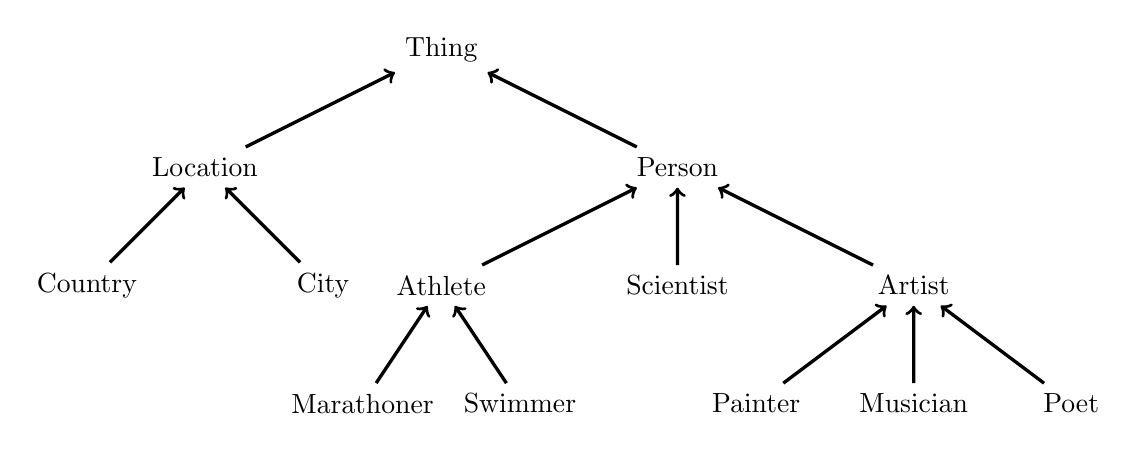
\begin{tikzpicture}[<-,draw=black,very thick,level/.style={sibling distance = 6cm/#1,level distance = 1.5cm}]
    
    \node{Thing}
      child{node {Location} 
	child{node {Country}}
	child{node {City}}
      }
      child{node {Person}
	child{node {Athlete}
	  child{node {Marathoner}}
	  child{node {Swimmer}}
	}
	child{node {Scientist}}
	child{node {Artist}
	  child{node {Painter}}
	  child{node {Musician}}
	  child{node {Poet}}
	}
      };
  \end{tikzpicture}
  \label{fig:hierarchy}
\end{figure}

We assume that the knowledge base has its type hierarchy described with the relation \emph{rdfs:subClassOf}, like in
the example shown in Figure~\ref{fig:hierarchy}, where each arrow means that the tail is a subclass of the head (e.g.,
Country is a subclass of Location). Also, we assume that every property has both argument types declared with
\emph{rdfs:domain} and \emph{rdfs:range}. With this information, it is a straightforward task to identify the pairs of
joining relations which are not allowed by the type hierarchy.    

For every pair of relations, we simply try to match the argument types from the two joining arguments. We
check whether the types are equal, or if one can be subsumed by the other, i.e., one is a subclass of the other. If so,
then the pair of relations is allowed to be joined on the given arguments. The pseudo-code for performing this task is
shown in Algorithm~\ref{alg1}:

\begin{algorithm}[h!]
  \caption{Function $checkTypes$ \newline Checks whether two relations are joinable for a given join pattern}
 \SetKwFunction{subsumes}
 \KwIn{\textbf{Input:} $r_i$, $r_j$: Joining relations, $arg_i$, $arg_j$: Joining arguments \\}
 \KwOut{True if $arg_i$ from $r_i$ joins with $arg_j$ from $r_j$, False otherwise}
  \Switch{$arg_i$} {
      \Case{$1$}{
	$type_i \leftarrow r_i.domain$\;
      }
      \Case{$2$}{
	$type_i \leftarrow r_i.range$\;
      }
  }
  \Switch{$arg_j$} {
      \Case{$1$}{
	$type_j \leftarrow r_j.domain$\;
      }
      \Case{$2$}{
	$type_j \leftarrow r_j.range$\;
      }
  }
  \eIf{$type_i = type_j$ {\bf or} \FuncSty{isSubClassOf(}$type_i$,$type_j$\FuncSty{)} {\bf or}
       \FuncSty{isSubClassOf(}$type_j$,$type_i$\FuncSty{)}}{
      \Return true\;
   }{
    \Return false\;
  }
 \label{alg1}
\end{algorithm}

It might happen that in the knowledge base, the cardinality of a join is zero or less than
the support threshold. Therefore, it is worth testing it beforehand, as we show in the next section.

\subsubsection{Exploiting Support Monotonicity}

In top-down ILP, support is a monotonically decreasing measure. As a result, we know that by adding any
literals to the hypothesis, we can only get a smaller or equal support. Therefore, we can query in the knowledge base
the cardinality of a join, and check whether it satisfies the support threshold or not.

If a given join does not reach the minimum support, we know that a clause containing this join will cannot reach it
either, so we can automatically prune this clause in the core ILP algorithm.

\begin{algorithm}[h!]
  \caption{Function $checkSupport$ \newline Checks whether join support exceeds threshold}
  \SetKwFunction{executeQuery}
  \KwIn{\textbf{Input:} $r_i$, $r_j$: Joining relations, $arg_i$, $arg_j$: Joining arguments, $supportThreshold$:
Support threshold \\ }
  \KwOut{True if join support exceeds threshold, False otherwise}
    \Switch{$(arg_i,arg_j)$} {
      \Case{$(1,1)$}{
	$query \leftarrow$ \emph{``select count distinct $?x$ where \{ $?x$ <$r_i$> $?y$ . $?x$ <$r_j$> $?z$ \}''}\;
      }
      \Case{$(1,2)$}{
	$query \leftarrow$ \emph{``select count distinct $?x$ where \{ $?x$ <$r_i$> $?y$ . $?z$ <$r_j$> $?x$ \}''}\;
      }
      \Case{$(2,1)$}{
	$query \leftarrow$ \emph{``select count distinct $?x$ where \{ $?y$ <$r_i$> $?x$ . $?x$ <$r_j$> $?z$ \}''}\;
      }
      \Case{$(2,2)$}{
	$query \leftarrow$ \emph{``select count distinct $?x$ where \{ $?y$ <$r_i$> $?x$ . $?z$ <$r_j$> $?x$ \}''}\;
      }
      \Case{$(11,22)$}{
	$query \leftarrow$ \emph{``select count distinct $?x$ $?y$ where \{ $?x$ <$r_i$> $?y$ . $?x$ <$r_j$> $?y$ \}''}
	\;
      }
      \Case{$(12,21)$}{
	$query \leftarrow$ \emph{``select count distinct $?x$ $?y$ where \{ $?x$ <$r_i$> $?y$ . $?y$ <$r_j$> $?x$ \}''}
	\;
      }
    }
    $joinSupport \leftarrow$ executeQuery($query$)\;
     \eIf{$joinSupport \ge supportThreshold$} {
      \Return true\;
    }{
      \Return false\;
    }
  \label{alg2}
\end{algorithm}


The preprocessing is done by Algorithm~\ref{alg3}, which uses Algorithm~\ref{alg1} in order to check if
the relation argument types match, and Algorithm~\ref{alg2} in order to test if the resulting join satisfies the
support threshold. With them, we can extract all the valid join combinations, and build 6 joining maps, one for each
join pattern. Each map has a relation as key, and a set of joinable relations as value. In the refinement step at the
ILP algorithm, these maps are queried in order to use set of valid literals relations in the subsequent refinements.

\begin{algorithm}[h!]
  \caption{Preprocessing algorithm}
  \SetKwFunction{executeQuery}
  \KwIn{\textbf{Input:} $r$: Set of Relations, $supportThreshold$: The support threshold \\ }
  \KwResult{$L_{m,n}(r_i)$: List of joinable relations, where $m,n \in \{1,2\}, r_i \in r$}

    \tcp{Lists initialization}
    \ForEach{$r_i \in r$} {
      $L_{1,1}(r_i) \leftarrow r_i$\;
      $L_{2,2}(r_i) \leftarrow r_i$\;
      $L_{11,22}(r_i) \leftarrow r_i$\;
      $L_{1,2}(r_i) \leftarrow \emptyset$\;
      $L_{2,1}(r_i) \leftarrow \emptyset$\;
      $L_{12,21}(r_i) \leftarrow \emptyset$\;
    }
    \tcp{For every possible pair of relations}
    \ForEach{$r_i \in r$} {
	\ForEach{$r_j \in r$ {\bf and} $j \geq i$} {
	    \If{$checkTypes(r_i,r_j,1,1)$ {\bf and} $checkSupport(r_i,r_j,1,1)$} {
		$L_{1,1}(r_i) \leftarrow L_{1,1}(r_i) \cup r_j$\;
		$L_{1,1}(r_j) \leftarrow L_{1,1}(r_j) \cup r_i$\;
	    }
	    \If{$checkTypes(r_i,r_j,2,2)$ {\bf and} $checkSupport(r_i,r_j,2,2)$} {
		$L_{2,2}(r_i) \leftarrow L_{2,2}(r_i) \cup r_j$\;
		$L_{2,2}(r_j) \leftarrow L_{2,2}(r_j) \cup r_i$\;
	    }
	    \If{$checkTypes(r_i,r_j,1,2)$ {\bf and} $checkSupport(r_i,r_j,1,2)$} {
		$L_{1,2}(r_i) \leftarrow L_{1,2}(r_i) \cup r_j$\;
		$L_{2,1}(r_j) \leftarrow L_{2,1}(r_j) \cup r_i$\;
	    }
	    \If{$checkTypes(r_i,r_j,2,1)$ {\bf and} $checkSupport(r_i,r_j,2,1)$} {
		$L_{2,1}(r_i) \leftarrow L_{2,1}(r_i) \cup r_j$\;
		$L_{1,2}(r_j) \leftarrow L_{1,2}(r_j) \cup r_i$\;
	    }
	}
   }
   \ForEach{$r_i \in r$} {
	\ForEach{$r_j \in (L_{1,1}(r_i) \cap L_{2,2}(r_i))$} {
	    \If{$checkSupport(r_i,r_j,11,22)$} {
		$L_{11,22}(r_i) \leftarrow L_{11,22}(r_i) \cup r_j$\;
	    }
	}
	\ForEach{$r_j \in (L_{1,2}(r_i) \cap L_{2,1}(r_i))$} {
	    \If{$checkSupport(r_i,r_j,12,21)$} {
		$L_{12,21}(r_i) \leftarrow L_{12,21}(r_i) \cup r_j$\;
	    }
	}
   }
  \label{alg3}
\end{algorithm}

\section{Correlation Lattice}
\label{sec:correlation-lattice}

During the preprocessing step, we build a graph inspired in the itemset lattice that represents the
correlations between various categories and a given numerical attribute. We call such graph a
correlation lattice.
Comparing to an itemset lattice, in a correlation lattice we have a set of categorical properties (defined in
Section~\ref{sec:categorical-properties}) instead of items. In addition, each node in the graph has an associated
frequency histogram which indicates its support distribution over the root's numerical attribute.

To illustrate this concept, let's analyze a simple real-world example extracted from the U.S.
Census\footnote{\url{http://www.rdfabout.com/demo/census/}} data, with the $hasIncome(X,Y)$ property. We analyze two
categorical relations: one strongly correlated to income, such as $hasEducation$, and one uncorrelated (or very
weakly correlated), such as $quarterOfBirth$.

For the relation $quarterOfBirth(X,Z)$, we have the 4 year quarters as possible constants for $Z$:

\begin{center}
  \begin{tabular}{r l}
    Q1:& January, February, March \\
    Q2:& April, May, June \\
    Q3:& July, August, September \\
    Q4:& October, November, December \\
  \end{tabular}
\end{center}

and for the relation $hasEducation(X,W)$, we have 16 different educational levels as possible constants for $W$:

\begin{center}
  \begin{tabular}{l l}
    	
    No school completed			&High school graduate                 		\\
    Nursery school to grade 4   	&Some college, less than 1 year			\\
    Grade 5 or grade 6          	&One or more years of college, no degree	\\
    Grade 7 or grade 8          	&Associate's degree				\\
    Grade 9                     	&Bachelor's degree				\\
    Grade 10                    	&Master's degree				\\
    Grade 11                    	&Professional school degree			\\
    Grade 12 no diploma 		&Doctorate degree				\\
  \end{tabular}
\end{center}

It's expected that the income distribution will be roughly the same for people born in any of the four year quarters,
whereas for different educational levels, the income distributions are
expected to be significantly different. 

\begin{figure}[h!]
\caption{Discrete probability distributions of income by year quarter (left), and by educational level (right)}
\begin{center}
  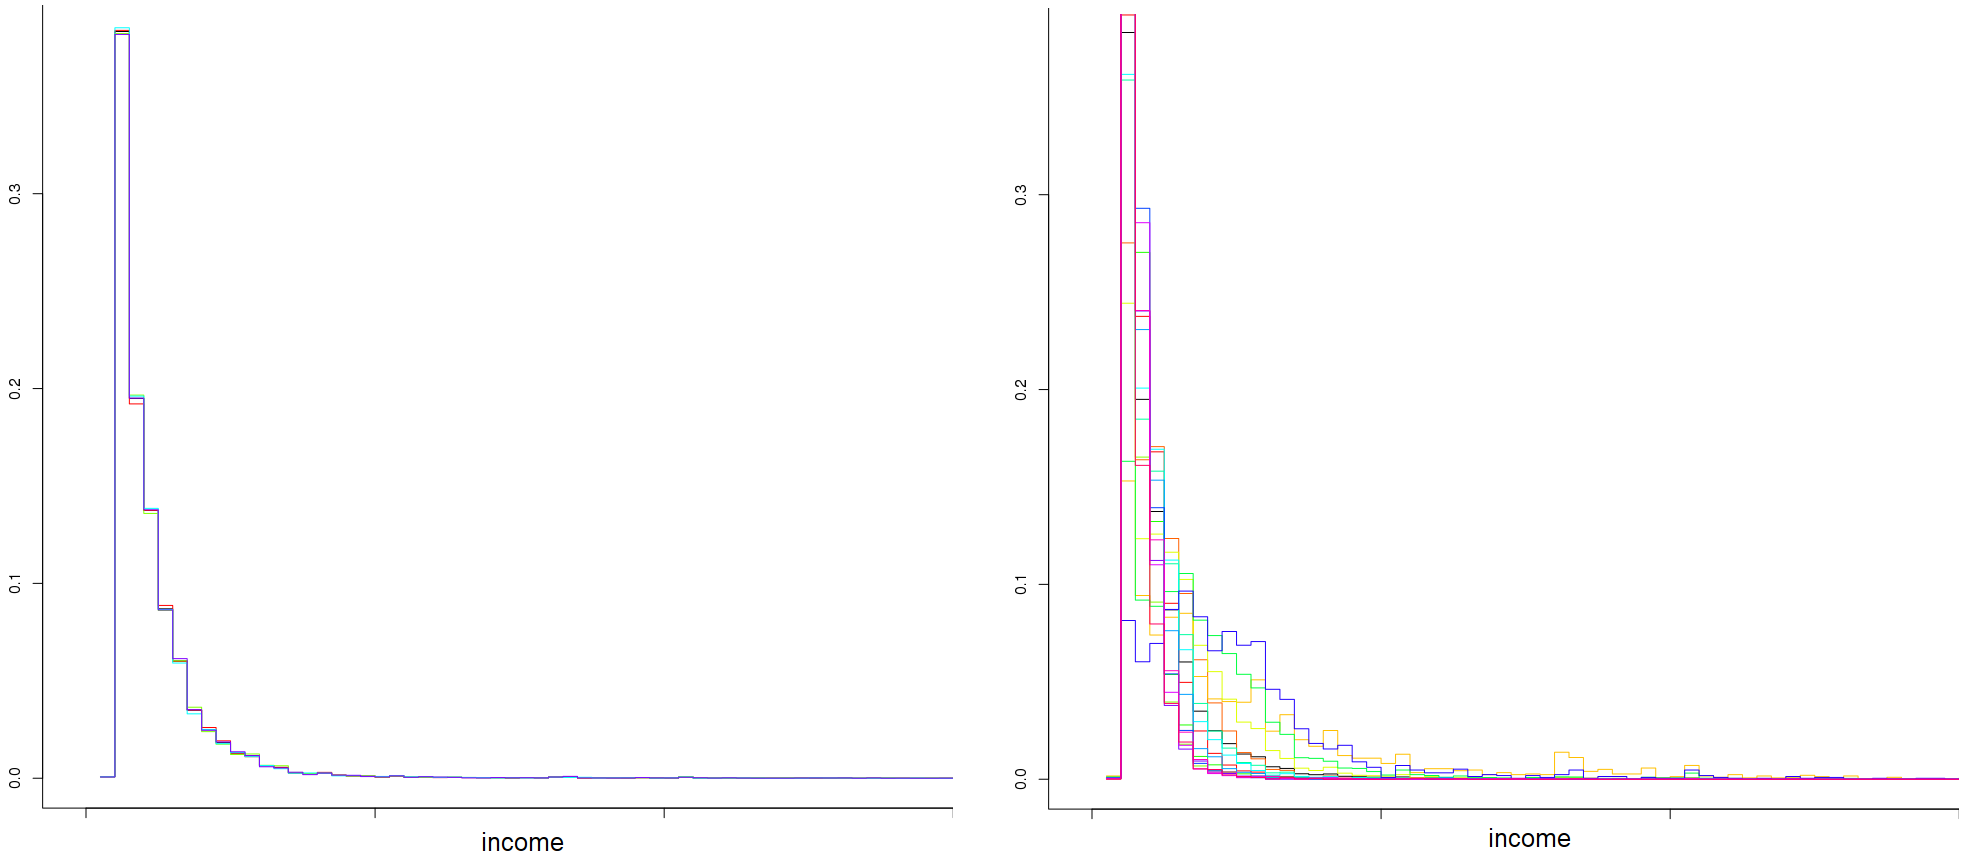
\includegraphics[width=1\linewidth]{./Figures/birthquarter-education.png}
\end{center}
\label{fig:income-education}
\end{figure}

Figure~\ref{fig:income-education} shows the discrete probability distributions of income in each category. On the left,
we have the four income distributions of people born in Q1, Q2, Q3 and Q4, and on the
right, the 16 different income distributions of people having each educational level. As it is easily noticeable, for
all the 4 year quarters, the income distribution is pretty much the same, while for the educational level, which has
great influence on the income, the distributions are very different.

\begin{figure}[h!]
\caption{Income distribution of the overall population, and the educational level categories: ``Nursery school to grade
4'' and ``Professional school degree''.}
\begin{center}
  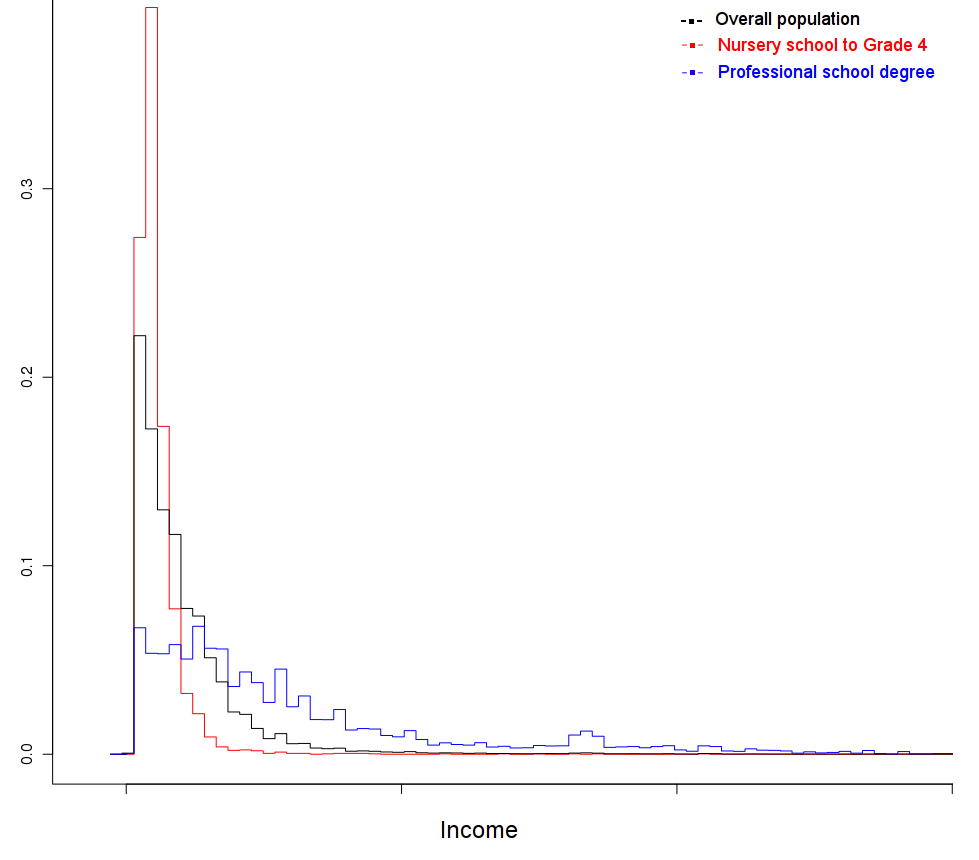
\includegraphics[width=0.7\linewidth]{./Figures/prof-nurs.png}
\end{center}
\label{fig:prof-nurs}
\end{figure}

In Figure~\ref{fig:prof-nurs}, we isolate two very distinct educational levels from Figure~\ref{fig:income-education}
(right): ``Nursery school to grade 4'' and ``Professional school degree''. The graph shows that in the first category,
there is relatively much more rich people, and much less poor people than in the latter.

Based on this idea, we check how different categorical relations affect a distribution by using divergence measures.
This information, together with other measures such as support, provides valuable insight about the interestingness of
adding a literal to a clause.


\subsection{Building the Lattice}

We start with the chosen numerical property, for example $hasIncome(X,Y)$, which should have at least two
arguments, one being a joining variable $X$, and the other the numerical attribute variable $Y$. Firstly, we query the
overall distribution along the numerical attribute $Y$, and discretize $Y$'s domain into $k$ buckets $b_1, b_2,
\dots, b_k$ using an unsupervised discretization method to define their boundaries. 

Afterwards, we build the frequency histogram of the root node for the defined buckets. We define the histogram of a
node $n$ over a numerical attribute variable $Y$ as a $k$-dimensional vector $h(n)$:

\begin{equation}
 h(n)=<h_1(n),h_2(n),\ldots,h_k(n)>
\end{equation}

where $h_i(n)=supp(n|Y \in b_i)$, and therefore:

\begin{equation}
  |h(n)|_1=\sum_{i=1}^{k}h_i(n)=supp(n)
\end{equation}

Every node in the lattice is composed by a conjunctive clause of non-negated literals and contains a frequency
histogram. For the sake of comparison, all histograms are built on the same buckets boundaries defined in the
root node. 

Subsequently, we do the same with the sub-populations defined by the chosen categorical properties. For each category, a
node in the lattice is created with the associated frequency histogram, and the new node is assigned as child of the
root node.

In a further step, we try to create further subcategories by joining intersecting categories. For example, with the
relations \emph{hasEducation} and \emph{quarterOfBirth}, we would then create the nodes:

  \emph{hasIncome(X,Y),quarterOfBirth(X,``Q1''),hasEducation(X,``Preschool'')} \newline
  \emph{hasIncome(X,Y),quarterOfBirth(X,``Q1''),hasEducation(X,``Kindergarten'')} \newline
  \centerline{\vdots} 
  \emph{hasIncome(X,Y),quarterOfBirth(X,``Q1''),hasEducation(X,``Doctorate Degree'')} \newline

  \centerline{\vdots} 

  \emph{hasIncome(X,Y),quarterOfBirth(X,``Q4''),hasEducation(X,``Preschool'')} \newline
  \emph{hasIncome(X,Y),quarterOfBirth(X,``Q4''),hasEducation(X,``Kindergarten'')} \newline
  \centerline{\vdots} 
  \emph{hasIncome(X,Y),quarterOfBirth(X,``Q4''),hasEducation(X,``Doctorate Degree'')} \newline


 \begin{figure}[!h]
  \caption{Combination of relations $hasEducation$ and $bornInMonth$ }
  \centering
  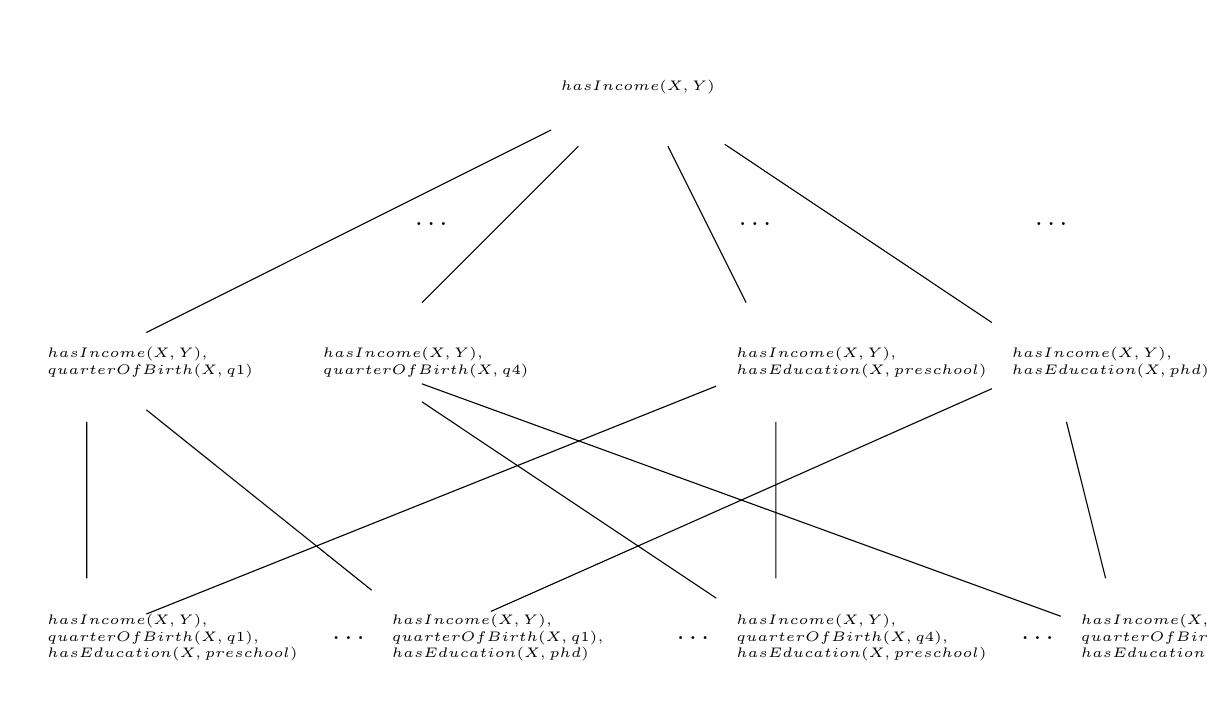
\begin{tikzpicture}[scale=1.75,auto=center,every node/.style={,minimum size=1.5cm,font=\tiny}]
    \node (r) 	at (5,5)  {$hasIncome(X,Y)$};
    \node[rectangle,text width=1cm,align=center] (a1) 	at (1,3) {$hasIncome(X,Y),$\\$quarterOfBirth(X,q1)$};
    \node[rectangle,text width=1cm,align=center] (an)	at (3,3) {$hasIncome(X,Y),$\\$quarterOfBirth(X,q4)$};
    \node[rectangle,text width=1cm,align=center] (b1)	at (6,3) {$hasIncome(X,Y),$\\$hasEducation(X,preschool)$};
    \node[rectangle,text width=1cm,align=center] (bm)	at (8,3) {$hasIncome(X,Y),$\\$hasEducation(X,phd)$};
    \node[font=\normalfont] (da)	at (3.5,4) {$\dots$};
    \node[font=\normalfont] (db)	at (5.85,4) {$\dots$};
    \node[font=\normalfont] (dn)	at (8,4) {$\dots$};
    \node[font=\normalfont] (d1)	at (2.9,1) {$\dots$};
    \node[font=\normalfont] (d2)	at (5.4,1) {$\dots$};
    \node[font=\normalfont] (d3)	at (7.9,1) {$\dots$};

    \node[rectangle,text width=1cm,align=center] (a1b1) 	at (1.0,1)
{$hasIncome(X,Y),$\\$quarterOfBirth(X,q1),$\\$hasEducation(X,preschool)$};
    \node[rectangle,text width=1cm,align=center] (a1bm)	at (3.5,1)
{$hasIncome(X,Y),$\\$quarterOfBirth(X,q1),$\\$hasEducation(X,phd)$};
    \node[rectangle,text width=1cm,align=center] (anb1) 	at (6.0,1)
{$hasIncome(X,Y),$\\$quarterOfBirth(X,q4),$\\$hasEducation(X,preschool)$};
    \node[rectangle,text width=1cm,align=center] (anbm)	at (8.5,1)
{$hasIncome(X,Y),$\\$quarterOfBirth(X,q4),$\\$hasEducation(X,phd)$};
    \foreach \from/\to in
      {r/a1,r/an,r/b1,r/bm,a1b1/a1,a1b1/b1,a1bm/a1,a1bm/bm,anb1/an,anb1/b1,anbm/an,anbm/bm}  
    \draw (\from) -- (\to);
  \end{tikzpicture}
  \label{fig:combiningLiterals}
\end{figure}

This process works just like in an itemset lattice until either a predetermined maximum level is reached, or until all
the possible combinations are exhausted. Figure~\ref{fig:lattice} shows how a correlation lattice looks like.

\begin{figure}[!h]
  \caption{Correlation Lattice example}
  \centering
  \begin{tikzpicture}
  [scale=1.8,auto=center,every node/.style={draw=black, font=\tiny}]
  \begin{tikzpicture}
 [scale=1.8,auto=center,every node/.style={minimum, font=\tiny}]
  \node (n0) at (4,10) {$r$};
  \node (na) at (0,8)  {$r a$};
  \node (na1)%[fill=blue!20] 
  at (1,7.5)  {$r a_1$};
  \node (na2)%[fill=blue!20] 
  at (2,7.5) {$r a_2$};
  \node (nb) at (3,8)  {$r b$};
  \node (nb1)%[fill=red!20] 
  at (4,7.5)  {$r b_1$};
  \node (nb2)%[fill=red!20] 
  at (5,7.5)  {$r b_1$};
  \node (nc) at (6,8)  {$r c$};
  \node (nc1)%[fill=green!20] 
  at (7,7.5)  {$r c_1$};
  \node (nc2)%[fill=green!20] 
  at (8,7.5)  {$r c_1$};
  \node (nab) at (0,5)  {$r a b$};
  \node (na1b1)%[fill=magenta!20] 
  at (0.5,4.5)  {$r a_1 b_1$};
  \node (na1b2)%[fill=magenta!20] 
  at (1.0,4.5)  {$r a_1 b_2$};
  \node (na2b1)%[fill=magenta!20] 
  at (1.5,4.5)  {$r a_2 b_1$};
  \node (na2b2)%[fill=magenta!20] 
  at (2.0,4.5)  {$r a_2 b_2$};
  \node (nac) at (3,5)  {$r a c$};
  \node (na1c1)%[fill=cyan!20] 
  at (3.5,4.5)  {$r a_1 c_1$};
  \node (na1c2)%[fill=cyan!20] 
  at (4.0,4.5)  {$r a_1 c_2$};
  \node (na2c1)%[fill=cyan!20] 
  at (4.5,4.5)  {$r a_2 c_1$};
  \node (na2c2)%[fill=cyan!20] 
  at (5.0,4.5)  {$r a_2 c_2$};
  \node (nbc) at (6,5)  {$r b c$};
  \node (nb1c1)%[fill=yellow!50] 
  at (6.5,4.5)  {$r b_1 c_1$};
  \node (nb1c2)%[fill=yellow!50] 
  at (7.0,4.5)  {$r b_1 c_2$};
  \node (nb2c1)%[fill=yellow!50] 
  at (7.5,4.5)  {$r b_2 c_1$};
  \node (nb2c2)%[fill=yellow!50] 
  at (8.0,4.5)  {$r b_2 c_2$};
  \node (nabc) at (2,2)  {$r a b c$};
  \node (na1b1c1)%[fill=black!10] 
  at (2.5,1.5)  {$r a_1 b_1 c_1$};
  \node (na1b1c2)%[fill=black!10] 
  at (3.2,1.5)  {$r a_1 b_1 c_2$};
  \node (na1b2c1)%[fill=black!10] 
  at (3.9,1.5)  {$r a_1 b_2 c_1$};  
  \node (na1b2c2)%[fill=black!10] 
  at (4.6,1.5)  {$r a_1 b_2 c_2$};
  \node (na2b1c1)%[fill=black!10] 
  at (5.3,1.5)  {$r a_2 b_1 c_1$};
  \node (na2b1c2)%[fill=black!10] 
  at (6.0,1.5)  {$r a_2 b_1 c_2$};
  \node (na2b2c1)%[fill=black!10] 
  at (6.7,1.5)  {$r a_2 b_2 c_1$};
  \node (na2b2c2)%[fill=black!10] 
  at (7.4,1.5)  {$r a_2 b_2 c_2$};

  \foreach \from/\to in {na/na1,na/na2,nb/nb1,nb/nb2,nc/nc1,nc/nc2}
    \draw[dashed] (\from) -| (\to);

  \foreach \from/\to in {nab/na1b1,nab/na1b2,nab/na2b1,nab/na2b2}
    \draw[dashed] (\from) -| (\to);

  \foreach \from/\to in {nabc/na1b1c1,nabc/na1b1c2,nabc/na1b2c1,nabc/na1b2c2,nabc/na2b1c1,nabc/na2b1c2,nabc/na2b2c1,nabc/na2b2c2}
    \draw[dashed] (\from) -| (\to);

  \foreach \from/\to in {n0/na1,n0/na2,na1/na1b1,na1/na1b2,na2/na2b1,na2/na2b2,na1/na1c1,na1/na1c2,na2/na2c1,na2/na2c2}
    \draw[blue] (\from) -- (\to);
  \foreach \from/\to in {n0/nb1,n0/nb2,nb1/na1b1,nb1/na2b1,nb2/na1b2,nb2/na2b2,nb1/nb1c1,nb1/nb1c2,nb2/nb2c1,nb2/nb2c2}
    \draw[red] (\from) -- (\to);
  \foreach \from/\to in {n0/nc1,n0/nc2,nc1/na1c1,nc1/na2c1,nc2/na1c2,nc2/na2c2,nc1/nb1c1,nc1/nb2c1,nc2/nb1c2,nc2/nb2c2}
    \draw[green] (\from) -- (\to);
  \foreach \from/\to in {na1b1/na1b1c1,na1b2/na1b2c1,na2b1/na2b1c1,na2b2/na2b2c1,na1b1/na1b1c2,na1b2/na1b2c2,na2b1/na2b1c2,na2b2/na2b2c2}
    \draw[magenta] (\from) -- (\to);
  \foreach \from/\to in {na1c1/na1b1c1,na1c1/na1b2c1,na2c1/na2b1c1,na2c1/na2b2c1,na1c2/na1b1c2,na1c2/na1b2c2,na2c2/na2b1c2,na2c2/na2b2c2}
    \draw[cyan] (\from) -- (\to);
  \foreach \from/\to in {nb1c1/na1b1c1,nb2c1/na1b2c1,nb1c1/na2b1c1,nb2c1/na2b2c1,nb1c2/na1b1c2,nb2c2/na1b2c2,nb1c2/na2b1c2,nb2c2/na2b2c2}
    \draw[yellow] (\from) -- (\to);

  \foreach \from/\to in {n0/na,n0/nb,n0/nc}
    \draw[dashed] (\from) -- (\to);
  \foreach \from/\to in {na/nab,na/nac,nb/nab,nb/nbc,nc/nac,nc/nbc,nab/nabc,nac/nabc,nbc/nabc}
    \draw[dashed] (\from) -- (\to);  
\end{tikzpicture}

  \end{tikzpicture}
  \label{fig:lattice}
\end{figure}

\subsection{Bucketing the Numerical Attribute}

The root's numerical attribute should be discretized by splitting its domain into a finite set of buckets in
order to build frequency histograms and compare distributions. In this section, we discuss about how to perform
such discretization.

The bucket boundaries used throughout the whole correlation lattice should be consistent. The bucketing method
as well as the boundaries are specified in the very beginning with the overall population defined by the root node. In
addition, they require as input an user-defined parameter $k$, which defines the number of buckets in all histograms.

Since we do not consider any labels for the examples, we use one of the unsupervised discretization methods presented
in Section~\ref{sec:rw-discretization}: equal frequencies or equal width. Equal frequencies is typically a safe choice
since it is less vulnerable to outliers and skewed distributions. On the other hand, equal width is simpler and less
expensive, being a good choice when the data is not very noisy and the numerical domain is well known.

\subsection{Pruning Opportunities}

In this Section we talk about pruning opportunities that can be exploited whilst building the correlation
lattice. As they might not be sufficient to reduce the lattice size to a feasible
level, later, in Section~\ref{sec:heuristics}, we also discuss possible heuristic pruning techniques.

\subsubsection{Support}

As described in~\citet{LavracDz94}, in top-down ILP, every refinement causes the support to decrease, therefore we
know that for every node in the correlation lattice, its support will be greater or equal than any of its children.
Hence, since support is a monotonically decreasing measure, we can use apriori-style pruning, which is also used in
ILP's refinement graph and association rule mining, and safely prune any node which does not satisfy the minimum
support threshold.

In this thesis, we define support as the absolute frequency of supporting facts. So the support of a node $n$ is
defined as:

\begin{center}
$supp(n)=|{x|x \in n}|$ 
\end{center}


\subsubsection{Independence Checks}
\label{sec:indepchecks}

By simplicity, we assume that every possible pair of categorical relations are independent given their common parent,
and we search for evidence to prove the contrary.

For 2 nodes to be joined, they must have a common parent, i.e., two nodes at level $l$ (with $l+1$ literals) are
joinable if they share $l$ literals. Therefore, it is simple to calculate the conditional probabilities of each
of the joining nodes given the common parent, and estimate the frequency distribution for the conditional independence
case.

%Let's say we have the following join case:
 
\begin{figure}[!h]
  \caption{Node join example for independence test}
  \centering
  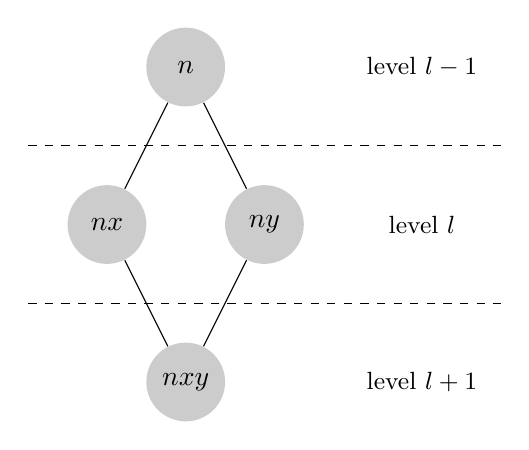
\begin{tikzpicture}
  [scale=1,auto=center,every node/.style={minimum size=1cm}]
    \node (p)  [circle,fill=black!20] at (4,10) {$n$};
    \node (n1) [circle,fill=black!20] at (3,8)  {$nx$};
    \node (n2) [circle,fill=black!20] at (5,8)  {$ny$};
    \node (n12)[circle,fill=black!20] at (4,6)  {$nxy$};

    \foreach \from/\to in {p/n1,p/n2,n1/n12,n2/n12}
      \draw (\from) -- (\to);

    \draw[dashed] (2,9) -- (8,9);
    \draw[dashed] (2,7) -- (8,7);

    \node (level0)[font=\small] at (7,10) {level $l-1$};
    \node (level1)[font=\small] at (7,8)  {level $l$};
    \node (level2)[font=\small] at (7,6)  {level $l+1$};
  \end{tikzpicture}
  \label{fig:joinIndepExample}
\end{figure}

In the example shown in Figure~\ref{fig:joinIndepExample}, $x$ and $y$ are literals and $n$ is a node with clause
$c_n$,
such that $x \neq y$ and $x,y \not \in c_n$. The nodes $nx$ and $ny$ are formed by adding $x$ and $y$ to $n$, so
$c_{nx}=\{c_n,x\}$ and $c_{ny}=\{c_n,y\}$. With the histogram from these three nodes, we can calculate the conditional
probability $p_i(x|n)$ and $p_i(y|n)$, then calculate $\hat{h_i}(nxy)$, which is the estimation of
$h_i(nxy)$ assuming that $x$ and $y$ are independent given common parent $n$.

\begin{align*}
 p_i(x|ny) &= p_i(x|n) \\ 
 &= \cfrac{h_i(nx)}{h_i(n)} \\ 
 p_i(y|nx) &= p_i(y|p) \\ 
 &= \cfrac{h_i(ny)}{h_i(n)} \\ \\ 
 \hat{h_i}(nxy) &= p_i(x|ny)p_i(y|n)h_i(n) \\ 
 &= p_i(x|p)h_i(yp) \\ 
 \hat{h_i}(nxy) &= p_i(y|nx)p_i(x|n)h_i(n) \\ 
 &= p_i(y|n)h_i(xn)
\label{eq:condindep}
\end{align*}

After that, we query the actual frequency distribution on the knowledge base and perform a Pearson's chi-squared
independence test. As null hypothesis and alternative hypothesis we have:

\begin{itemize}
 \item $H_0$ = \emph{$x$ and $y$ are conditionally independent given their common parent $p$}
 \item $H_1$ = \emph{$x$ and $y$ are conditionally dependent given their common parent $p$} 
\end{itemize}

the number of degrees of freedom is the number of buckets minus one:

\begin{center}
 $df=k-1$
\end{center}

and the critical value $\chi^2$ is calculated by:

\begin{equation}
 \chi^2=\sum_{i=1}^{k} \cfrac{(h_i - \hat{h_i})^2}{\hat{h_i}}
\end{equation}

with that it is possible to obtain the p-value, and check whether there is enough confidence to reject the null
hypothesis $H_0$. 

In other words, if we find out that $x$ and $y$ are conditionally independent given $p$, we could infer the
equivalences below, with equivalent rules having significantly similar confidence distributions:

\begin{center}
  $x$:-$p,y \equiv x$:-$p \quad$ and  $\quad y$:-$p,x \equiv y$:-$p$
\end{center}

Therefore, we know that if we have $x$ fixed as the head in the core ILP, and $x$:-$p$ as the current
clause, joining the node $px$ with $py$ to obtain the rule $x$:-$p,y$ does not add any valuable information. The same
principle applies for having $y$ as head, and obtaining $y$:-$p,x$ from $y$:-$p$ by joining the same pair of nodes. This
property plays an important role in the literal suggestion for clause refinements, as we explain in
more details in Section~\ref{sec:incorporation}.

This idea is very similar to the idea of the lift measure (presented in Section~\ref{sec:rw-arm}) of detecting
attributes independence. However, as we also take into account the support distribution, we use a more sophisticated
technique that compares the observed and expected distribution assuming independence.

\begin{comment}
In level 1 from \graphname, nodes can be directly pruned, on the other hand, for further levels, for a node to be
pruned by independence, all the possible joins resulting the node must be independent. In level 2, for example, in
order
to prune the node $r a_1 b_1 c_1$, given that in level 1 the nodes $r a_1 b_1$, $r a_1 c_1$ and $r b_1 c_1$ were not
pruned. All the three possible join combinations should fail the independence test, i.e.:

\begin{equation}
\begin{split} 
  freq(r a_1 b_1 c_1) &\approx freq(r a_1)p (r b_1|r a_1) p(r c_1|r a_1) \\ 
  &\approx  freq(r b_1) p(r a_1|r b_1) p(r c_1|r b_1) \\ 
  &\approx  freq(r c_1) p(r a_1|r c_1) p(r b_1|r c_1)  
\end{split}
\end{equation}
\end{comment}

This applies to nodes at any level $l$, with $p \leq l$ parents and $C_{2}^{p}$ possible join pairs. If any of the
join pairs has enough evidence of being dependent, then the resulting node is added as child of the two joining nodes.
If a given node is independent from all possible join pairs of parent nodes, one could eventually prune the node,
however, as we show later, it is not safe.

\begin{comment}
THIS IS REDUNDANT!!! (ALREADY DISCUSSED IN INTERESTINGNESS MEASURE)
\subsection{Entropy Divergence Measures}

As seen in the previous sections, we are interested in rules whose base-rule has accuracy below threshold, but
contains one or multiple specific intervals with accuracy above the threshold. For this to happen, we need a rule with
non-uniform accuracy distribution, or in other words, divergent body support and rule positive examples distributions.

Therefore, we are interested in adding categories that produces distributions different from their parent nodes'. In
order to measure such divergence between distributions, some of the state-of-the-art such as the following ones can be
used.

\begin{itemize}
 \item Kullback-Leibler~\cite{Kullback51klDivergence}: 
    \begin{equation}
      D_{KL}(P||Q)=\sum_{\substack{i}}\ln\left(\cfrac{P(i)}{Q(i)}\right)P(i)
    \end{equation}
 %\item Chi-squared ($\chi^2$):
 %  \begin{equation}
 %    D_{\chi^2}(P||Q)=\sum_{\substack{i}}\cfrac{(P(i)-Q(i))^2}{P(i)}
 %  \end{equation}
 \item Jensen-Shannon~\cite{17795}:
    \begin{equation}
      D_{JS}(P||Q)=\cfrac{1}{2}D_{KL}(P||M)+\cfrac{1}{2}D_{KL}(Q||M), 
    \end{equation}
\end{itemize}

Where $P$ and $Q$ are discrete probability distributions to be compared and $M=\cfrac{1}{2}(P+Q)$. In the lattice
context, these distributions would be the frequency histogram normalized to 1, and nodes directly connected by edges
would have their distributions compared.

As discussed in Section~\ref{sec:kldiv}, although Jensen-Shannon is computationally more expensive, it has the advantage
of being a symmetric and smoothed version of the Kullback-Leibler measure. 

These divergence measures are important for identifying potential accuracy distributions. If the divergence between the
frequency distributions of a parent and child node is big, that means that if we have a rule with the parent node as
body and the additional literal from the child as head, its accuracy distribution will not be uniform and therefore
potentially be interesting for searching for refined-rules with numerical intervals.
\end{comment}

\subsection{Heuristics}
\label{sec:heuristics}

As seen before, the number of nodes in a correlation lattice grows exponentially with the number of categorical
relations and its constants. For $n$ categorical relations, each with $m$ constants, the total number of nodes is
$2^{nm}$. In this thesis, we limit the number of levels in the lattice to $l$, where $l$ is the maximum number of
literals allowed in a clause by the core-ILP. With this reduction, the total number of nodes is reduced from:

\begin{center}
  \begin{equation}
    \sum_{i=1}^{mn}\binom{nm}{i} = 2^{nm}
  \end{equation}
\end{center}

to a much smaller number, since typically $l \ll nm$:

\begin{center}
  \begin{equation}
    \sum_{i=1}^{l}\binom{nm}{i}
  \end{equation}
\end{center}

Pruning by support is usually not sufficient to make an exhaustive search feasible, therefore, it is necessary to apply
heuristics to prune it more aggressively.

%%% Divergence

Pruning by divergence is clearly not safe. Let's suppose we have a root numerical property $r(X,Y)$, and two
non-overlapping categorical relations $a(X,Z)$ with constants $z_1$ and $z_2$ and $b(X,W)$ with constants $w_1$ and
$w_2$. For simplicity, let's assume that the numerical variable $Y$ is divided into two buckets and root $r$ has an
uniform distribution frequency histogram $h(r)=<2,2>$ which results in the probability distribution $<0.5,0.5>$.

It is possible join $r$ with $a$ and $b$ obtaining the following uniform frequency histograms:

\begin{center}
$h(ra_1)=<1,1>$ \\
$h(ra_2)=<1,1>$ \\
$h(rb_1)=<1,1>$ \\
$h(rb_2)=<1,1>$
\end{center}

Although all of the nodes have the exact same probability distribution as $r$, which results in a divergence measure of
zero, they could not be safely pruned, since it is possible to have $r$, $a$, and $b$ combined with totally different
distributions that maximize the divergence measure:

\begin{center}
$h(ra_1b_1)=<1,0>$ \\
$h(ra_1b_2)=<0,1>$ \\
$h(ra_2b_1)=<0,1>$ \\
$h(ra_2b_2)=<1,0>$
\end{center}

As shown above, divergence is not a monotonically decreasing measure, since, for instance, we have $D_{JS}(r || ra_1) <
D_{JS}(ra_1 || ra_1b_1)$. Therefore, if we have an interesting measure composed by divergence and support, for example,
we can only heuristically prune uninteresting nodes.

% Draw example instead to explain better
\begin{comment}
Moreover, using a divergence measure alone might also be problematic. Histograms with low support are more likely to
present a higher divergence than histograms with higher support, supposing that they were drawn from the same original
distribution. That happens due to the sampling error, which says that smaller samples are more likely to have a
distribution more different to the original distribution from which it was drawn. Consequently, the exclusive use of
the divergence as heuristics would end up giving preference to nodes with lower support. Therefore, it is important to
use divergence combined with support as pruning heuristics.
\end{comment}
%Moreover, we are interested not only in rules with high confidence, but also rules with high support so more facts can
%be derived.

% Talk about how to use such measure? (Threshold, Top-k, Cost-Benefit)

%%% Independence

As seen in Section~\ref{sec:indepchecks}, checking for conditional independence of categories is very insightful
and can detect equivalent rules. Nevertheless, if for the example shown in Figure~\ref{fig:joinIndepExample} we find out
that $x$ and $y$ are conditionally independent given $p$, we cannot prune the node $pxy$ from the lattice since $x$ and
$y$ might not be independent given $p,z$, and and in such case, the rule $x$:-$p,y,z$ would not be equivalent to
$x$:-$p,y$, and therefore eventually interesting.

However, the obtained p-value is still a very insightful measure, and can be used as heuristics for reducing the
number of nodes in the lattice.

\section{Incorporating Correlation Lattice into the Core ILP Algorithm}
\label{sec:incorporation}

The ILP core learning algorithm requires some modifications in order to support the correlation lattice. As stated
before, we use top-down search, starting from the most general clauses then further refining them by introducing
new substitutions or literals until a stopping criteria is reached.

\subsection{Querying the Correlation Lattice}
\label{sec:queryingTheLattice}

In the ILP refinement loop, the head literal is fixed. As the head literal plays fundamental role in the
interestingness of a clause, this literal should be included in the correlation lattice. If so, once the root literal
of a correlation lattice is added to a clause in the refinement loop, and this clause satisfies the support threshold,
we can query this lattice in order to predict whether the clause is interesting or not, as well as get a list of
literal suggestions to be added to the clause in the next refinement step.

For getting the list of suggestions, the first step would be to search in the lattice the literals already present in
both head and body that are joined with the root literal, and then search for the child nodes with
highest interestingness. Nevertheless, we are not interested in the benefit of adding a literal to the conjunction
of rule's head and body, but in the benefit of adding the head to the body refined with a new literal.

For example, if we have the clause $a$:-$r$, where $r$ is the root of a correlation lattice and the head $a$ is included
in it. After searching in the graph for the literals joined with root present in the clause we would come to node
$ra$. We are not searching for the most interesting child from $ra$, but for the children, which has a parent without
the head literal that has the has the highest interestingness measure when adding the head.

\begin{figure}[!h]
  \caption{Interestingness of adding a literal to the body}
  \centering
  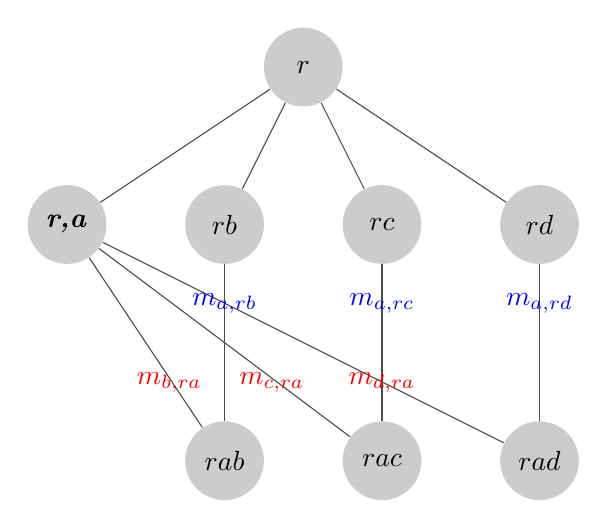
\begin{tikzpicture}
  [scale=1,auto=center,every node/.style={minimum size=1cm}]
    \node (r)  [circle,fill=black!20] at (4,10) {$r$};
    \node (ra) [circle,fill=black!20] at (1,8)  {\textbf{\emph{r,a}}};
    \node (rb) [circle,fill=black!20] at (3,8)  {$rb$};
    \node (rc) [circle,fill=black!20] at (5,8)  {$rc$};
    \node (rd) [circle,fill=black!20] at (7,8)  {$rd$};
    \node (rab)[circle,fill=black!20] at (3,5)  {$rab$};
    \node (rac)[circle,fill=black!20] at (5,5)  {$rac$};
    \node (rad)[circle,fill=black!20] at (7,5)  {$rad$};

    \foreach \from/\to in {r/ra,r/rb,r/rc,r/rd,ra/rab,ra/rac,ra/rad,rb/rab,rc/rac,rd/rad}
      \draw[black!70] (\from) -- (\to);

    \node (m1)[blue] at (3,7)  {\textbf{$m_{a,rb}$}};
    \node (m2)[blue] at (5,7)  {$m_{a,rc}$};
    \node (m3)[blue] at (7,7)  {$m_{a,rd}$};
    \node (m4)[red] at (2.3,6)  {$m_{b,ra}$};
    \node (m5)[red] at (3.6,6)  {$m_{c,ra}$};
    \node (m6)[red] at (5.0,6)  {$m_{d,ra}$};

    %\draw (ra) -- (rab) -|  \node [below,pos=0.25] {$m_1$}(l1);
  \end{tikzpicture}
  \label{fig:latticeSuggestion}
\end{figure}

This example is illustrated in Figure~\ref{fig:latticeSuggestion}, if we can add $b$, $c$ or $d$ to $ra$, we are
interested in the measures $m_{a,rb}$, $m_{a,rc}$ and $m_{a,rd}$ (shown in blue), instead of $m_{b,ra}$, $m_c,ra$ and
$m_{d,ra}$ (shown in red). Nevertheless, searching for values of $m_{a,rb}$, $m_{a,rc}$ and $m_{a,rd}$ is a bit tricky.
It is necessary to check for all children of $ra$, which have parents without head literal $a$, then gather all the
interestingness measures of the head in relation to the body and sort.

In order to avoid visiting multiple nodes, we can create suggestions maps when the lattice is built. These map
contain an entry for all node it is joined to, with head as key, and a refinement suggestions list sorted by
measure as value. So for example when we are creating the node $rab$ by joining $ra$ and $rb$, we add to $ra$ an entry
with $a$ as key, $b$ as new literal and  associated measure $m_{a,rb}$ and we also add to $rb$ an entry with $b$ as key,
$a$ as new literal and associated measure $m_{b,ra}$. This is shown more clearly in Algorithm~\ref{alg:buildmaps}.

\begin{algorithm}[h!]
 \caption{Suggestion map build when joining nodes during lattice build}
 \KwIn{\textbf{Input:} $nx, ny$: Joining nodes, $n$: Common parent node}
  $\hat{h}(nxy) \leftarrow h(nx)h(ny)/h(n)$\;
  $h(nxy) \leftarrow $\FuncSty{queryFrequencyHistogram(}$nxy$\FuncSty{)}\;
  $\chi^2 \leftarrow \sum_{i=1}^{k}(h_i(nxy)-\hat{h}_i(nxy))^2/(\hat{h}_i(nxy))$\;
  $dof \leftarrow k-1$\;
  $pValue = $\FuncSty{criticalValue(}$\chi^2,dof$\FuncSty{)}\;
  \If{$pValue \geq minPValue$}{
    $m_{x,ny} \leftarrow $\FuncSty{interestingness(}$h(nxy),h(ny)$\FuncSty{)}\;
    $m_{y,nx} \leftarrow $\FuncSty{interestingness(}$h(nxy),h(nx)$\FuncSty{)}\;
    $nx.suggestions(x) \leftarrow (y,m_{x,ny})$\;
    $ny.suggestions(y) \leftarrow (x,m_{y,nx})$\;
  }
 \label{alg:buildmaps}
\end{algorithm}

In the example of Figure~\ref{fig:latticeSuggestion}, $ra$ would contain the following map with a single entry for the
only possible head literal $a$:

\begin{center}
  \begin{tabular}{r | l}
    a & b [$m_{a,rb}$] \\
      & c [$m_{a,rc}$] \\
      & d [$m_{a,rd}$]
  \end{tabular}
\end{center}

Below, we have the map from the node $ra_1b_1$ from the example shown in Figure~\ref{fig:lattice}, in this case it has
two entries for each possible head literal: $a_1$ and $b_1$: 

\begin{center}
  \begin{tabular}{r | l}
    a1 	& c1 [$m_{a_1,rb_1c_1}$] \\
	& c2 [$m_{a_1,rb_1c_2}$] \\
    \hline
    b1	& c1 [$m_{b_1,ra_1c_1}$] \\
	& c2 [$m_{b_1,ra_1c_2}$]
  \end{tabular}
\end{center}

More generally speaking, for a node at level $l$ with $l+1$ literals (one of them being the root), we can have up to $l$
keys in the map. Therewith, we can much more easily find the best suggestions for any possible head literal without
having to visit other nodes.

First we need to introduce the search for numerical intervals as a possible refinement in the top-down ILP refinement
step. This refinement would be possible only if the body contains a literal which is the root of a correlation
lattice and whose numerical attribute variable is free, as shown in Algorithm~\ref{alg4}. If so, then we can try to
predict whether the clause is interesting by calling the function \FuncSty{predictInterestingness}, which is shown
in Algorithm~\ref{alg6}. This function simply queries the interestingness of adding the current clause's head to its
body, and checks whether it satisfies the specified interestingness threshold.

\begin{algorithm}[h!]
 \caption{Extension to the refinement step}
 \SetKwFunction{checkNumericalRanges}
 \KwIn{\textbf{Input:} $clause$: Set of literals from the clause, $lattice(r_{root})$: Set of existent Correlation
Lattices, 
 $lit_{body}$: Literal in clause that will be joined with new Literal, $lit_{new}$: Literal to be added to the clause,
 $arg_{body}$: Join argument from body literal, $arg_{new}$: Join argument from new literal, $interestingnessThreshold$:
Minimum interestingness value allowed \\}
 
  $r_{new} \leftarrow lit_{new}.relation$\;
  \If{$arg_{new} = 1$ \textbf{and} $r_{new}$ is numerical \textbf{and} $\exists$ $lattice(r_{new})$} {
    $root \leftarrow$ $lattice(r_{new}).root$\;
    \If{\FuncSty{predictInterestingness(}$clause$,$root$,$interestingnessThreshold$\FuncSty{)}} {
	\FuncSty{checkNumericalRanges(}$clause$,$lit_{new}$,$node$\FuncSty{)}\;
    }
  }
 \label{alg4}
\end{algorithm}

\begin{algorithm}[!h]
 \caption{\FuncSty{checkNumericalRanges}}
 \SetKwFunction{queryAccuracyDistribution, querySupportDistribution}
 \KwIn{\textbf{Input:}  \\}
 \KwOut{}
  $v \leftarrow $ Numerical variable from $lit_{new}$\;
  $acc \leftarrow $ \FuncSty{queryConfidenceDistribution(}$clause$,$v$\FuncSty{)}\;
  $sup \leftarrow $ \FuncSty{querySupportDistribution(}$clause$, $v$\FuncSty{)}\;
  $intervals \leftarrow $  \FuncSty{searchInterestingIntervals(}$acc$,$sup$,$accTS$,$supTS$\FuncSty{)}\;
  \ForEach{$interval_i \in intervals$} {
     $newClause \leftarrow \{clause \cup lit_{new} \cup \{v \in interval_i\}\}$\;
     Add $newClause$ to ILP's refinement graph\;
  }
  $suggestions \leftarrow node.getSuggestions(clause.head)$\;
  \ForEach{$lit_i \in suggestions$ \textbf{and} $i \leq k$} {
    $node_i \leftarrow node$.\FuncSty{search(}$lit_i$\FuncSty{)}\;
    \FuncSty{checkNumericalRanges(}$clause \cup lit_i$,$lit_{new}$,$node_i$\FuncSty{)}\;
  }
 \label{alg5}
\end{algorithm}

\begin{algorithm}[!h]
 \caption{\FuncSty{predictInterestingness}}
 \SetKwFunction{checkNumericalRanges}
 \KwIn{\textbf{Input:} $clause$: Clause with numerical literal, $root$: Correlation lattice root node,
$interestingnessThreshold$: Minimum interestingness value allowed }
  $bodyNode \leftarrow root$\;
  \ForEach{$lit_i \in clause.body$} {
    $bodyNode \leftarrow bodyNode$.\FuncSty{search(}$lit_i$\FuncSty{)}\;
  }
  $headNode \leftarrow bodyNode$.\FuncSty{search(}$clause.head$\FuncSty{)}\;
  \eIf{$headNode \neq bodyNode$} {
      $interestingness \leftarrow
      $\FuncSty{measureInterestingness(}$headNode.distribution$,$bodyNode.distribution$\FuncSty{)}\;
      \If{$interestingness \geq interestingnessThreshold$} {
	  \Return true\;
      }
  } {
      \Return  false\;
  }
 \label{alg6}
\end{algorithm}

Once we find out that the clause is interesting, we can perform the numerical interval search refinement
shown in Algorithm~\ref{alg5}. It basically queries the support and confidence distribution of the base-rule along the
numerical attribute and searches for optimal intervals using techniques, such as \cite{Brin99miningoptimized}, presented
in Section~\ref{sec:rw-miningOptimizedRules}, and which is represented in Algorithm~\ref{alg4} by the function
\FuncSty{searchInterestingIntervals}. If any relevant interval is found, we add the required arithmetic literals to
restrict the numerical variable domain and add the clause to the ILP's refinement graph. Subsequently, the
algorithm also queries the correlation lattice for suggestion of new literals to be added to the clause


\section{Searching Rules in Correlation Lattice}
\label{sec:searchRulesInCL}

In the lattice itself, it is possible to extract valuable rules. Given its characteristic of all the relations being
joined on the same root argument, these extracted rules represent how different categories are related along root's
numerical constants.

Every non-root node in the correlation lattice can be the body of a rule, and the new literal from any of
its children the head. 

Below, we show an example using the notation defined at~\ref{sec:notation}. For the node $r a_1 b_1$ with children $r
a_1 b_1 c_1$, $r a_1 b_1 c_2$ and $r a_1 b_1 d_1$, we can easily evaluate three rules:
\begin{align*}
Rule_1: \quad &c_1\text{ :- }a_1,b_1,r \\ 
&supp(Rule_1) = h(r a_1 b_1 c_1) \\
&acc(Rule_1) = \frac{h(r a_1 b_1 c_1)}{h(a_1,b_1,r)}% \\ \\
\end{align*}
\begin{align*}
Rule_2: \quad &c_2\text{ :- }a_1,b_1,r \\
 &supp(Rule_2) = h(r a_1 b_1 c_2) \\
 &acc(Rule_2) = \frac{h_i(r a_1 b_1 c_2)}{h(a_1,b_1,r)} %\\ \\
\end{align*}
\begin{align*}
Rule_3: \quad &d_1\text{ :- }a_1,b_1,r \\
 &supp(Rule_3) = h(r a_1 b_1 d_1) \\
 &acc(Rule_3) = \frac{h(r a_1 b_1 d_1)}{h(a_1,b_1,r)} 
\end{align*}

Therefore, in order to search for rules in the correlation lattice, we can simply perform a breadth-first traversal in
the lattice, and this such evaluation for every node. 

Subsequently we can analyze the frequency and confidence distributions and determine whether any of the rules are
interesting, using any of the techniques such as \citet{Brin99miningoptimized}, discussed
in Section~\ref{sec:rw-miningOptimizedRules}, in order to search for optimal intervals.
